\begin{center}
    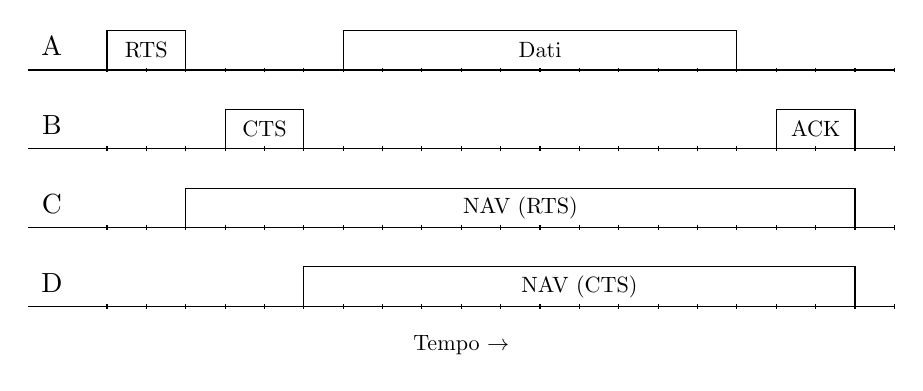
\begin{tikzpicture}
        %%%%%%%%%% Assi %%%%%%%%%%
        \foreach \y in {0,...,3}
            \draw (0,\y) -- ++(11,0);

        \node at (.3,3.3) {A};
        \node at (.3,2.3) {B};
        \node at (.3,1.3) {C};
        \node at (.3,0.3) {D};

        \foreach \y in {-0.03,.97,...,2.97}
            \foreach \x in {1,1.5,...,11}
                \draw (\x,\y) -- ++(0,.06);

        %%%%%%%%% Blocchi %%%%%%%%
        \draw (1,3) -- ++(0,.5) -- ++(1,0) -- ++(0,-0.5);
        \draw (4,3) -- ++(0,.5) -- ++(5,0) -- ++(0,-0.5);
        \draw (2.5,2) -- ++(0,.5) -- ++(1,0) -- ++(0,-0.5);
        \draw (9.5,2) -- ++(0,.5) -- ++(1,0) -- ++(0,-0.5);
        \draw (2,1) -- ++(0,.5) -- ++(8.5,0) -- ++(0,-0.5);
        \draw (3.5,0) -- ++(0,.5) -- ++(7,0) -- ++(0,-0.5);

        %%%%%%%%% Testo %%%%%%%%%%
        \node[scale=0.8] at (1.5,3.25) {RTS};
        \node[scale=0.8] at (6.5,3.25) {Dati};
        \node[scale=0.8] at (3,2.25) {CTS};
        \node[scale=0.8] at (10,2.25) {ACK};
        \node[scale=0.8] at (6.25,1.25) {NAV (RTS)};
        \node[scale=0.8] at (7,.25) {NAV (CTS)};
        \node[scale=0.8] at (5.5,-0.5) {Tempo $\rightarrow$};
    \end{tikzpicture}
\end{center}